\documentclass[12pt, oneside]{book}
\usepackage{graphicx}  % this is for includegraphics

\usepackage{setspace}
\onehalfspacing % this sets spacing to 1.5 


\usepackage{amsmath}
\usepackage{amsthm} % for theorems, lemmas etc
\usepackage{amsfonts}
\usepackage{lipsum} % to generate the lipsum random text in the sample
\usepackage{tikz}
\usepackage{siunitx}

\usetikzlibrary{calc,decorations.pathmorphing,patterns}


\usepackage[colorlinks=true, urlcolor=blue, pdfborder={0 0 0}]{hyperref}
\hypersetup{
     colorlinks   = true,
     citecolor    = blue
}

\theoremstyle{plain}
\newtheorem{theorem}{Theorem}[section]
\newtheorem{proposition}[theorem]{Proposition}
\newtheorem{lemma}[theorem]{Lemma}
\newtheorem{corollary}[theorem]{Corollary}
\newtheorem{fact}[theorem]{Fact}

\theoremstyle{definition}
\newtheorem{definition}[theorem]{Definition}
\newtheorem{example}[theorem]{Example}
\newtheorem{remark}[theorem]{Remark}
\newtheorem{remarks}[theorem]{Remarks}

\newcommand{\Cov}{\mathrm{Cov}}
\newcommand{\Var}{\mathrm{Var}}

\begin{document}

\begin{titlepage}
\begin{center}
        \vspace{-2cm}
Mathematical Finance MSc Dissertation MTH775P, 2018/19 
		\\
        \Huge
        \textbf{Accelerated Grids}
        \\        
        \vspace{0.4cm}
        \LARGE
        Optimizing Solvers for Financial Partial Differential Equations
        \\        
        \vspace{0.4cm}        
        \textbf{Mustafa Berke Erdis, ID 180883925}% student name and number        
        \\
        \large Supervisor: Dr. Sebastian del Bano Rollin
        \\
        \vspace{0.9cm}
        
\includegraphics[scale=0.23]{QMCrest.png}
        \\
        \vspace{0.9cm}        
        \LARGE 
        A thesis presented for the degree of\\
        Master in Sciences in \emph{Mathematical Finance}\\
        \vspace{0.7cm}        
        \Large
        School of Mathematical Sciences\\ 
        and \emph{School of Economics and Finance}\\
        Queen Mary University of London \\
    \end{center}
\end{titlepage}


\chapter*{Declaration of original work}
\begin{flushright}
This declaration is made on \today.
\end{flushright}


{\bf Student's Declaration:}
I, Mustafa Berke Erdis, hereby declare that the work in this thesis 
is my original work. I have not copied from any other students' work, work of 
mine submitted elsewhere,  or from any other sources except where due reference or acknowledgement is made explicitly in the text, nor has any part been written for me by another person.

Referenced text has been flagged by:
\begin{enumerate}
\item Using italic fonts, {\bf and} % LaTeX: {\it text}  
\item using quotation marks ``\ldots '', {\bf and}
\item explicitly mentioning the source in the text.
\end{enumerate}

%This excludes any definitions known from your modules or undethat can be found in an undergraduate text book.

\newpage

\thispagestyle{empty}
        \begin{flushright}
                This work is dedicated to my family.
        \end{flushright}
\vspace{\stretch{2}}\null



\chapter*{Acknowledgements}
Here you thank people that have helped you in the journey. \\
\lipsum[100] % replace this by your text

\chapter*{Abstract}
\begin{center}
\small 
Here you write a short summary, around 10 lines, of your work. \\
\lipsum[100]% replace this by your text
\end{center}       


\chapter*{Preface}
Here  you write a summary of the work. A paragraph on the motivation, previous work, then maybe a brief chapter by chapter summary. 

\lipsum[100]% replace this by your text



\begin{flushright}
Queen Mary University of London\\
12${}^{\text{th}}$ August 2019
\end{flushright}


\tableofcontents

\chapter{Introduction}
In Ancient Greece, Thales was scorned for his poverty. Later that year, Thales utilized his skills in astrology. He forecasted the increase in olive yields. Using his limited capital, he rented oil presses in winter. Over the oil making season, many people rushed to the presses because of the high yields. Thales, as he rented the presses over the winter, let them upon what terms he pleased. Thales showed it was easy for philosophers to be rich if they chose it and accidentally laid the foundations of financial derivatives. \cite{Thalesians}

In the modern world, financial derivatives are contracts between two or more parties. The value of the contract depends on one or several underlying assets. Commonly the assets are currencies, equities, bonds, interest rates, market indices or commodities.

The simplest vanilla call option the right but not the obligation to buy the underlying at the expiry date at a previously agreed strike price. Thales essentially bought call options for oil presses.  So if the olive yields didn't come as Thales expected he didn't have the obligation to use the olive presses.

\section{Pricing Financial Derivatives}\label{Pricing Financial Derivatives}
\subsection{The Risk Neutral Approach}
\begin{definition} Brownian Motion 

Brownian motion (also known as Wiener Process) was discovered by botanist Robert Brown as he observed a chaotic motion of particles suspended in water. \cite{BM}  A  Brownian  motion, $B(t)$,  is  a  continuous-time  stochastic  process  with  the  following properties: 
\begin{itemize}
\item $ B(0) = 0 $.
\item $ B(t) $ is a continuous function of t.
\item For $ 0  \leq s < t $ the increment $ B(t) -  B(s)  $ has normal distribution $ \mathcal{N}(0, t-s) $.
\end{itemize}
Brownian motion is the basic building block in stochastic calculus and geometric Brownian motion is often used to model the stock prices.

\end{definition}

\begin{theorem} It\^{o}'s Lemma

Let $B(t)$ be a Brownian motion and $W(t)$ be an Ito drift-diffusion process which satisfies the stochastic differential equation:
\begin{equation}
dW(t) = \mu(W(t),t)dt + \sigma(W(t),t)dB(t)
\end{equation} 
If $f(w, t) \in C^2(\mathbb{R}^2,\mathbb{R})$ then $f(W(t),t)$ is also an Ito drift-diffusion process, with its differential given by:
\begin{equation}
d(f(W(t),t)) = \frac{\partial f}{\partial t}(W(t),t)dt + f'(W(t),t)dW + \frac{1}{2}f''(W(t),t)dW(t)^2
\end{equation} 
With $dW(t)^2$ given by: $dt^2 = 0$, $dt dB(t) = 0$ and $dB(t)^2 = dt$.
\end{theorem}



\begin{theorem} Black-Scholes Model

The Black-Scholes framework is a theoretical valuation formula for options. Since almost all corporate liabilities can be viewed as combinations of options, the formula is applicable to common stock, corporate bonds etc.  \cite{BS} Under the assumptions of Black-Scholes framework, the call or put option price satisfies the parabolic partial differential equation:
\begin{equation}
\frac{\partial V}{\partial t} + \frac{1}{2}\sigma^2 S^2 \frac{\partial^2 V}{\partial S^2} = r(V - S \frac{\partial V}{\partial S})
\end{equation}

\end{theorem}  

\begin{proof} 

Suppose an investor sets up a self-financing portfolio at time t, with a total value $ X(t)$. 
The portfolio consists of:
\begin{itemize}
\item $ \Delta(t) $ share of stocks
\item Remaining $ X(t) - \Delta(t)S(t) $ deposit in the riskless bank account which yields continuously compounded interest at rate $r$.
 
\end{itemize}
Self-financing trading strategy has no capital influx or consumption, the value of portfolio changes as: 
\begin{equation}
dX(t) =  \Delta(t)dS(t) + r(X(t) +  \Delta(t)S(t))dt
\end{equation}

Black-Scholes model assumes that the stock price under the "market probability measure" follows a gBM. 

\begin{equation}
S(t) = S(0) exp((\alpha - \sigma^2/2)t + \sigma B(t)), t \geq 0
\end{equation} where $\sigma > 0$ is a constant volatility parameter, $ \alpha > 0$ is a mean rate of return. In differential form: 
\begin{equation}
dS(t) = \alpha S(t)dt + \sigma S(t)dB(t) 
\end{equation}

Putting (1.4) and (1.6) together yields
\begin{equation}
 dX(t) = rX(t)dt + (\alpha - r) \Delta(t)S(t)dt + \sigma \Delta(t)S(t)dB(t)
\end{equation}

The first term denotes the return on investment X(t) in bank, second term is the risk premium and third term appears due to the volatility of the stock market.

In order to calculate the differential for the discounted portfolio value $exp(-rt) X(t) $, we use the It\^{o}'s formula.

\begin{equation}
 d(exp(-rt) X(t)) = -r exp(-rt) X(t)dt + exp(-rt) dX(t)
 \end{equation}
 
 Substituting $dX(t)$ from (1.7)
 
 \begin{equation}
 (\alpha - r) \Delta(t)S(t)dt + \sigma \Delta(t)S(t)dB(t)
\end{equation}

\end{proof}

\begin{remark} 1 sayfa anlat bunu
The Black-Scholes model is still  used but not entirely applicable to assets that cannot be hedged. Multi asset derivatives(equity baskets), Weather derivatives, non tradable assets, not freely tradable FX (Brazil real, Korean Won). The industry uses a different product called non deliverable forward for such.
\end{remark}



\subsection{Solving Financial Partial Differential Equations}


Since the foundation of the world humanity tried to understand and model the nature. Differential equations serves this purpose by enabling us to describe natural phenomena for instance, heat, sound and fluid flow. The mathematical theory of partial differential equations describing financial markets plays an important role in mathematical finance.

General form of 2nd order PDEs of two independent variables is $$ au_{xx} + bu_{xy} + cu_{yy} + du_x + eu_y + fu + g = 0 $$ If the equation satisfies the condition $ b^2 - 4ac = 0 $  it is considered a parabolic partial differential equation. Generally, financial partial differential equations can be classified as parabolic partial differential equations.


Sometimes there are analytical solutions derive analytical bs/separation of variables heat equation Vanilla options barrier options reference (1 page)

Numerical partial differential equations is a large area of study. The subject includes components in the areas of applications, mathematics and computers. These three aspects of a problem are so strongly tied together that it is virtually impossible to consider the applied aspect of a problem without considering at least some of the mathematical counting aspects of that problem.[j.w. thomas]

On the other hand, mostly partial differential equations are too complicated to work out an analytical solution. Thus, we need to achieve a numerical solution to the problem.

The most common framework is finite difference method which tries to find approximate solutions to the problem at a discrete set of points, normally on a rectangular grid of points.
Instead we try to find approximate solutions of the problem at a discrete set of points in the (x, t) plane, normally a rectangular grid of points. It is simple to construct and analyse but can compromise performance because of increased computational complexity when there are high dimensions. 

But sometimes we need to use numerical methods Monte carlo high dimensions, Grids low dimensions show feynman kac writes as expectation
Glassermann MC book rough calculation of error MC vs PDE grids(1-2 pages)
Finally, the Monte Carlo method is used to find the numerical solution when dimensions are too high by calculating an expectation (Feynman-Kac Theorem) klebaner.

\section{Finite Difference Methods}
Parabolic partial differential equation can be denoted as
$$ \frac{\partial u}{\partial t} = a(t,x) \frac{\partial^2 u}{\partial x^2} + b(t,x) \frac{\partial u}{\partial x} + c(t,x) u(t,x) + d(t,x) $$

$a(t,x)$ denotes diffusion coefficient,  $b(t,x)$ convection coefficient, $c(t,x)$ reaction coefficient, $d(t,x)$ source coefficient.

1st order Central Difference 
$$ \frac{\partial u}{\partial x} = \frac{u^{n}_{i+1} - u^n_i}{\Delta t} $$

    \begin{figure}[!htb]
        \centering
            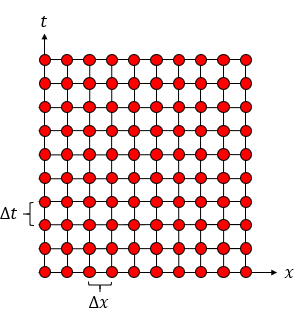
\includegraphics[scale=0.9]{Discretize.png}
        \caption{Discretizing on 10 x 10 grid}
    \end{figure}
    
Utilizing the boundary conditions and initial conditions:
    \begin{figure}[!htb]
        \centering
            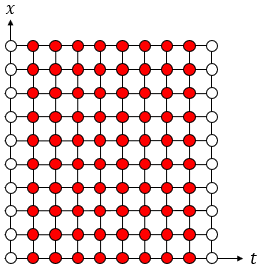
\includegraphics[scale=0.9]{Boundary.png}
        \caption{Applying the boundary conditions}
    \end{figure}

    \begin{figure}[!htb]
        \centering
            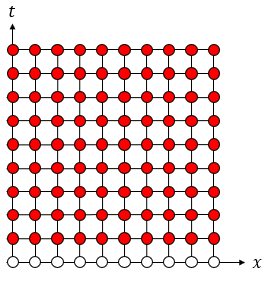
\includegraphics[scale=0.9]{Initial.png}
        \caption{Applying the boundary conditions}
    \end{figure}

\subsection{Explicit Method}
Explicit method is a forward time, central space scheme .
1st order Forward Difference
$$ \frac{\partial u}{\partial t} = \frac{u^{n+1}_i - u^n_i}{\Delta t} $$

2nd order Central Difference 
$$ \frac{\partial^2 u}{\partial x^2} = \frac{u^n_{i+1}- 2u^n_i + u^n_{i-1}}{(\Delta x)^2} $$

The parabolic partial differential equation can be generalized by applying the forward difference to the time derivative and the centred second difference.
$$ u_j^{n+1} = \alpha u_{j-1}^{n} + \beta u_{j}^{n} + \gamma u_{j+1}^{n} $$

For heat equation the coefficients become
$$ \alpha =  r, \beta = 1 - 2r, \gamma = r $$

Black-Scholes partial differential equation the coefficients become:
$$ \alpha =  \frac{\sigma^2 j^2 \Delta t}{2} - \frac{r j \Delta t}{2}, \beta = 1 - \sigma^2 j^2 \Delta t - r \Delta t, \gamma = \frac{\sigma^2 j^2 \Delta t}{2} - \frac{r j \Delta t}{2} $$

where $ r = \frac{\delta t}{\delta x^2} $.

    \begin{figure}[!htb]
        \centering
            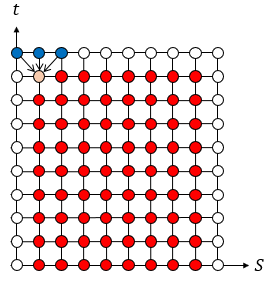
\includegraphics[scale=0.9]{Explicit.png}
        \caption{Computational stencil of explicit method}
    \end{figure}

\subsection{Crank-Nicholson Method}
The crank nicolson method was introduced \cite{cn}

$$ u(t,x) \approx \frac{1}{2} ( u^{n+1}_i +  u^n_i) $$

$$   \frac{\partial u}{\partial t} \approx \frac{u^{n+1}_i - u^n_i}{\Delta t} $$

$$   \frac{\partial u}{\partial x} \approx \frac{u^n_{i+1} - u^n_{i-1} + u^{n+1}_{i+1} - u^{n+1}_{i-1}}{4\Delta x} $$

$$ \frac{\partial^2 u}{\partial x^2} \approx \frac{u^n_{i+1}- 2u^n_i + u^n_{i-1} + u^{n+1}_{i+1}- 2u^{n+1}_i + u^{n+1}_{i-1}}{2(\Delta x)^2} $$

$$ A = a(t,x) \frac{\Delta t}{\Delta x^2},  B = b(t,x) \frac{\Delta t}{4\Delta x}, C = c(t,x) \frac{\Delta t}{2},  D = d(t,x) \Delta t $$ 



\begin{multline}
 (-A -B) u^{n+1}_{i+1} + (1 + 2A - C) u^{n+1}_i + (-A + B) u^{n+1}_{i-1} =  \\
=  (A+B) u^{n}_{i+1} + (1 - 2A + C) u^{n}_i + (A - B) u^{n}_{i-1} + D
\end{multline}





The left hand side groups the unknowns and the right hand side groups knowns. The system of equations can be represented by a tridiagonal matrix system. Most commonly these system are solved by Thomas Algorithm.

\begin{definition} Thomas Algorithm \\
The method is used to solve a tridiagonal matrix system invented by Llewellyn Thomas \cite{thomas}. The system equations can be written as
$$
\begin{bmatrix}  
b_1 & c_1 & 0 & 0 & ... & 0 \\ 
a_2 & b_2 & c_2 & 0 & ... & 0 \\ 
0 & a_3 & b_3 & c_3 & 0 & 0 \\ 
. & . &  &  &  & . \\ 
. & . &  &  &  & . \\ 
. & . &  &  &  & c_{k-1} \\ 
0 & 0 & 0 & 0 & a_k & b_k \\ 
\end{bmatrix} \begin{bmatrix}  
f_1 \\ 
f_2 \\ 
f_3 \\ 
.\\ 
.\\ 
.\\ 
f_k \\ 
\end{bmatrix} = \begin{bmatrix} 
d_1 \\ 
d_2 \\ 
d_3 \\ 
.\\ 
.\\ 
.\\ 
d_k \\ 
\end{bmatrix}
$$


The method begins by forming coefficients \(c^{*}_i\) and \(d^{*}_i\) in place of \(a_i\), \(b_i\) and \(c_i\) as follows:
$$
c^{*}_i = \left\{
     \begin{array}{lr}
       \frac{c_1}{b_1} & ; i = 1\\
       \frac{c_i}{b_i - c^{*}_{i-1} a_i} & ; i = 2,3,...,k-1
     \end{array}
   \right.
$$
$$   
d^{*}_i = \left\{
     \begin{array}{lr}
       \frac{d_1}{b_1} & ; i = 1\\
       \frac{d_i-d^{*}_{i-1} a_i}{b_i - c^{*}_{i-1} a_i} & ; i = 2,3,...,k-1
     \end{array}
   \right.
   $$
With these new coefficients, the matrix equation can be rewritten as:
$$
\begin{bmatrix}  
1 & c^{*}_1 & 0 & 0 & ... & 0 \\ 
0 & 1 & c^{*}_2 & 0 & ... & 0 \\ 
0 & 0 & 1 & c^{*}_3 & 0 & 0 \\ 
. & . &  &  &  & . \\ 
. & . &  &  &  & . \\ 
. & . &  &  &  & c^{*}_{k-1} \\ 
0 & 0 & 0 & 0 & 0 & 1 \\ 
\end{bmatrix} \begin{bmatrix}  
f_1 \\ 
f_2 \\ 
f_3 \\ 
.\\ 
.\\ 
.\\ 
f_k \\ 
\end{bmatrix} = \begin{bmatrix} 
d^{*}_1 \\ 
d^{*}_2 \\ 
d^{*}_3 \\ 
.\\ 
.\\ 
.\\ 
d^{*}_k \\ 
\end{bmatrix}
$$
The algorithm for the solution of these equations is now straightforward and works 'in reverse':

\[ f_k = d^{*}_k, \qquad f_i = d^{*}_k - c^{*}_i x_{i+1}, \qquad i = k-1, k-2, ... ,2,1 \]

\end{definition}

\subsection{Rannacher Trick}
Using the Crank nicholson 



\subsection{Alternating Direction Implicit Method}
The alternate direction implicit (ADI) method is used to numerically solve two dimensional parabolic PDEs. ADI schemes give us advantages of implicit finite difference method and computationally only requires to solve tridiagonal matrices.

ADI Peaceman and Rachford in 1955 \cite{peace}

Operator splitting is a natural and old idea. When a PDE or system of PDEs contains different terms expressing different physics, it is natural to use different numerical methods for different physical processes. This can optimize and simplify the overall solution process. The idea was especially popularized in the context of the Navier-Stokes equations and reaction-diffusion PDEs. Common names for the technique are operator splitting, fractional step methods, and split-step methods. We shall stick to the former name. In the context of nonlinear differential equations, operator splitting can be used to isolate nonlinear terms and simplify the solution methods.

A related technique, often known as dimensional splitting or alternating direction implicit (ADI) methods, is to split the spatial dimensions and solve a 2D or 3D problem as two or three consecutive 1D problems, but this type of splitting is not to be further considered here.


\begin{equation}
\delta x^2 u^{n}_{i,j}  = \frac{u^{n}_{i+1,j} - 2u^{n}_{i,j} + u^{n}_{i-1,j}}{\Delta x^2}
\end{equation}

\begin{equation}
\frac{u^{n+1}_{i,j} + u^{n}_{i,j}}{\Delta t} = \delta x^2 u^{n}_{i,j} + \delta y^2 u^{n}_{i,j}
\end{equation}

\begin{equation}
\frac{u^{n+1}_{i,j} + u^{n}_{i,j}}{\Delta t} = \delta x^2 u^{n+1}_{i,j} + \delta y^2 u^{n+1}_{i,j}
\end{equation}

Divide each time step in half
Implicit x, Explicit y:
\begin{equation}
\frac{u^{n+1/2}_{i,j} + u^{n}_{i,j}}{0.5 \Delta t} = \frac{\delta x^2 u^{n+1/2}_{i,j} }{\Delta x^2} + \frac{\delta y^2 u^{n}_{i,j}}{\Delta y^2}
\end{equation}

Explicit x, Implicit y:
\begin{equation}
\frac{u^{n+1}_{i,j} + u^{n+1/2}_{i,j}}{0.5 \Delta t} = \frac{\delta x^2 u^{n+1/2}_{i,j} }{\Delta x^2} + \frac{\delta y^2 u^{n+1}_{i,j}}{\Delta y^2}
\end{equation}


    \begin{figure}[!htb]
        \centering
            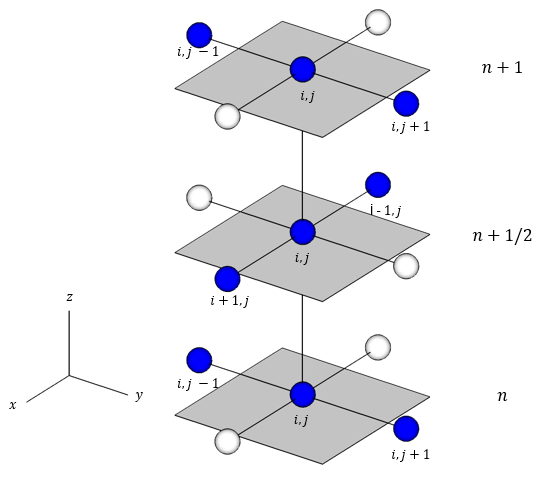
\includegraphics[scale=0.8]{ADI.png}
        \caption{Computational stencil of alternating direction implicit method}
    \end{figure}



\section{Optimizations}
Derivative pricing in the real world is a computationally intensive task. The existing numerical methods for partial differential equations are all constrained by the computational complexity. Being fast when evaluating new information is critical for the operations of hedge funds and investment banks. referansbul Therefore optimizing the existing numerical methods with hardware and software that can be installed on a trading floor is crucial. Main optimization techniques that can be implemented can be listed as follows.

\subsection{Compilers}
Intel Compiler, VS Compiler, gcc

\subsection{32 bit and 64 bit}

\subsection{Optimization Switches}

\subsection{Tridiagonal Solvers}
Thomas Algorithm, cyclic reduction double sweep.
\subsection{Threading}
High performance computing techniques that can be implemented for multithreading with Open Multi-Processing(OpenMP) and compiler intrinsics.
\subsection{OpenMP}
\subsection{AVX and Intrinsics}
CPUs are pipelining and use of SSE/SIMD kusswurm registers with Advanced Vector Extensions(AVX 512),
\subsection{GPGPU}
 In the case of General Purpose GPUs, CUDA or Open Computing Language(OpenCL) can be utilized but can be challenging because of the requirement of delicate memory management.

\subsection{Cloud Applications}

\chapter{Optimization of Financial PDEs}
First step is to write a simple version on a simple framework that can be calculated by hand and with Excel. Following the verifications, next step is porting the simple version in a high level programming language like python for prototyping and validating all calculations. The penultimate step is moving into a low level programming language such as C++ and utilize high performance computing principles.

Numerical analysis and computer simulations will be undertaken to put theory and observation together to gain insight into the workings of numerical solutions of partial differential equations.

Most basic case for parabolic differential equations is the heat equation
\begin{equation}
u_t(x,t)=u_{xx}(x, t)
\end{equation}
Initial Conditions
\begin{equation}
u(x, 0) = sin(\pi x)
\end{equation}
Boundary Conditions
\begin{equation}
u(0, t) = u(x_max, t) = 0
\end{equation}

Black-Scholes model for call option
\begin{equation}
\frac{\partial C}{\partial t} + \frac{1}{2}\sigma^2 S^2 \frac{\partial^2 C}{\partial S^2} = r(C - S \frac{\partial C}{\partial S})
\end{equation}
Initial Conditions
\begin{equation}
C(S, T) = (S - K, 0)^+
\end{equation}
Boundary Conditions
\begin{equation}
C(S_max, t) = S_max - K exp(-r(T-t))
C(0, t) = 0
\end{equation}

2 Dimensional Heat Equation to test ADI method:
\begin{equation}
\frac{\partial f}{\partial t} = \frac{\partial^2 f}{\partial x^2} +\frac{\partial^2 f}{\partial y^2}
\end{equation}
Initial Condition
\begin{equation}
f(x,y,0) = 1
\end{equation}
Boundary Conditions
\begin{equation}
f(x, 0, t) = f(x, 1, t) = 0
\end{equation}
\begin{equation}
f(x, 0, t) = f(x, 1, t) = 0
\end{equation}

\section{Timing the Code}
Measuring execution time intervals accurately is an important aspect to compare the efficiency and speed of different implementations.

\subsection{Windows API}

\subsection{Chrono Library}



\chapter{Conclusions}


\appendix
\chapter{Implementation of the {\tt FiniteDifferenceMethod} class}
\lipsum[10]
\chapter[shorter running title]{Additional details on the Gundermanian determinant}
\lipsum[10]


    

\bibliographystyle{plain}
\bibliography{ThesisDraft_v1}




\end{document}